% Volume I: Mathematical Language and Finite-Dimensional Geometry
% Continuity note for Chapter 1.
% Previous dependencies: none beyond arithmetic, reading formulas left to right, and comfort with small finite examples.
% New durable concepts: typed objects, statements, variables, parameters, assumptions, quantifiers, sets, relations, equivalence classes, proof methods, counterexamples, constructions, and models as lossy compressions.
% Forward hooks: Chapter 2 reuses the typed-object habit by treating functions as typed relationships between domains and codomains; later chapters reuse preimages, equivalence classes, proof templates, and model maps.
% Notation commitments: sets use uppercase letters such as X, Y, A, B, S, and Omega; elements use lowercase letters; parameters use theta in Theta; relations are subsets R of A times B; predicates are P(x); model predictions are m_theta(pi(omega)).
% Figure plan: four ImageGen raster figures are referenced: typed objects/statements for 1.1, relations/classes for 1.2, proof methods for 1.3, and modeling compression for 1.4.
\section{Chapter 1: Mathematical Language, Proof, and Abstraction}
\label{ch:mathematical-language-proof-abstraction}

This opening chapter begins before vectors, matrices, derivatives, or probability. It asks how mathematical language makes complex scientific and computational situations precise enough to reason about. A spike count, a stimulus, a parameter, a data set, a hypothesis, and a prediction are different kinds of things. Much of mathematical maturity begins with not letting those kinds blur.

The central problem of the chapter is this: how do we turn informal ideas into typed objects, meaningful statements, reliable proofs, and useful models without pretending that the notation is the reality? The answer is not a logic encyclopedia. It is a small working discipline: name the objects, state the assumptions, check the types, choose the proof method that matches the claim, and remember that every model compresses the world.

The chapter moves in four steps. Section 1.1 introduces objects, statements, notation, variables, parameters, and quantifiers. Section 1.2 builds sets and relations as the basic grammar for domains, predicates, and logical structure. Section 1.3 treats proof methods as practical tools for ruling out failure cases. Section 1.4 explains mathematical modeling as compression: a model keeps selected structure, discards other details, and earns its use by predicting or explaining something.

\subsection{1.1 Mathematical objects, statements, and notation}

\paragraph{Motivating question.}
When a formula contains symbols such as \(x\), \(r\), \(\theta\), \(X\), \(Y\), and \(f_\theta\), how do we know which expressions are meaningful statements and which are type errors?

\paragraph{Beginner setup.}
A \emph{mathematical object} is anything a theory is allowed to talk about: a number, a set, a vector, a function, a stimulus, a spike count, a parameter, or a probability distribution. A \emph{statement} is a sentence about objects that can be true or false once the objects and assumptions are fixed. A \emph{variable} names an object that may vary over an allowed collection. A \emph{parameter} names an object that is held fixed while we study variation in other objects. An \emph{assumption} states a condition under which later statements are meant to be read.

The smallest nontrivial example is a stimulus-response model. Let \(X\) be a set of stimuli, let \(Y=\{0,1,2,\ldots,K\}\) be a set of spike counts in a short time bin, and let \(\Theta\) be a set of possible parameter values. A model with parameter \(\theta\in\Theta\) may be written
\[
f_\theta:X\to Y.
\]
For an input \(x\in X\), the expression \(f_\theta(x)\) is meaningful and belongs to \(Y\). The expression \(f_\theta(r)\), where \(r\in Y\), is not meaningful unless \(Y\) is also allowed as an input set. That is a type error, not a deep falsehood.

This language solves a basic problem: it lets us separate data, model, parameter, output, and claim. In computation, this is the difference between a valid function call and an argument of the wrong shape. In mathematics, it is the difference between a statement that can be proved or refuted and a string of symbols that does not yet mean anything.

What to keep in mind: before asking whether a statement is true, ask whether it is well typed. A false statement has the right kind of objects but says something incorrect. An ill-typed expression tries to combine objects in a way the definitions do not permit.

\begin{figure}[htbp]
\centering
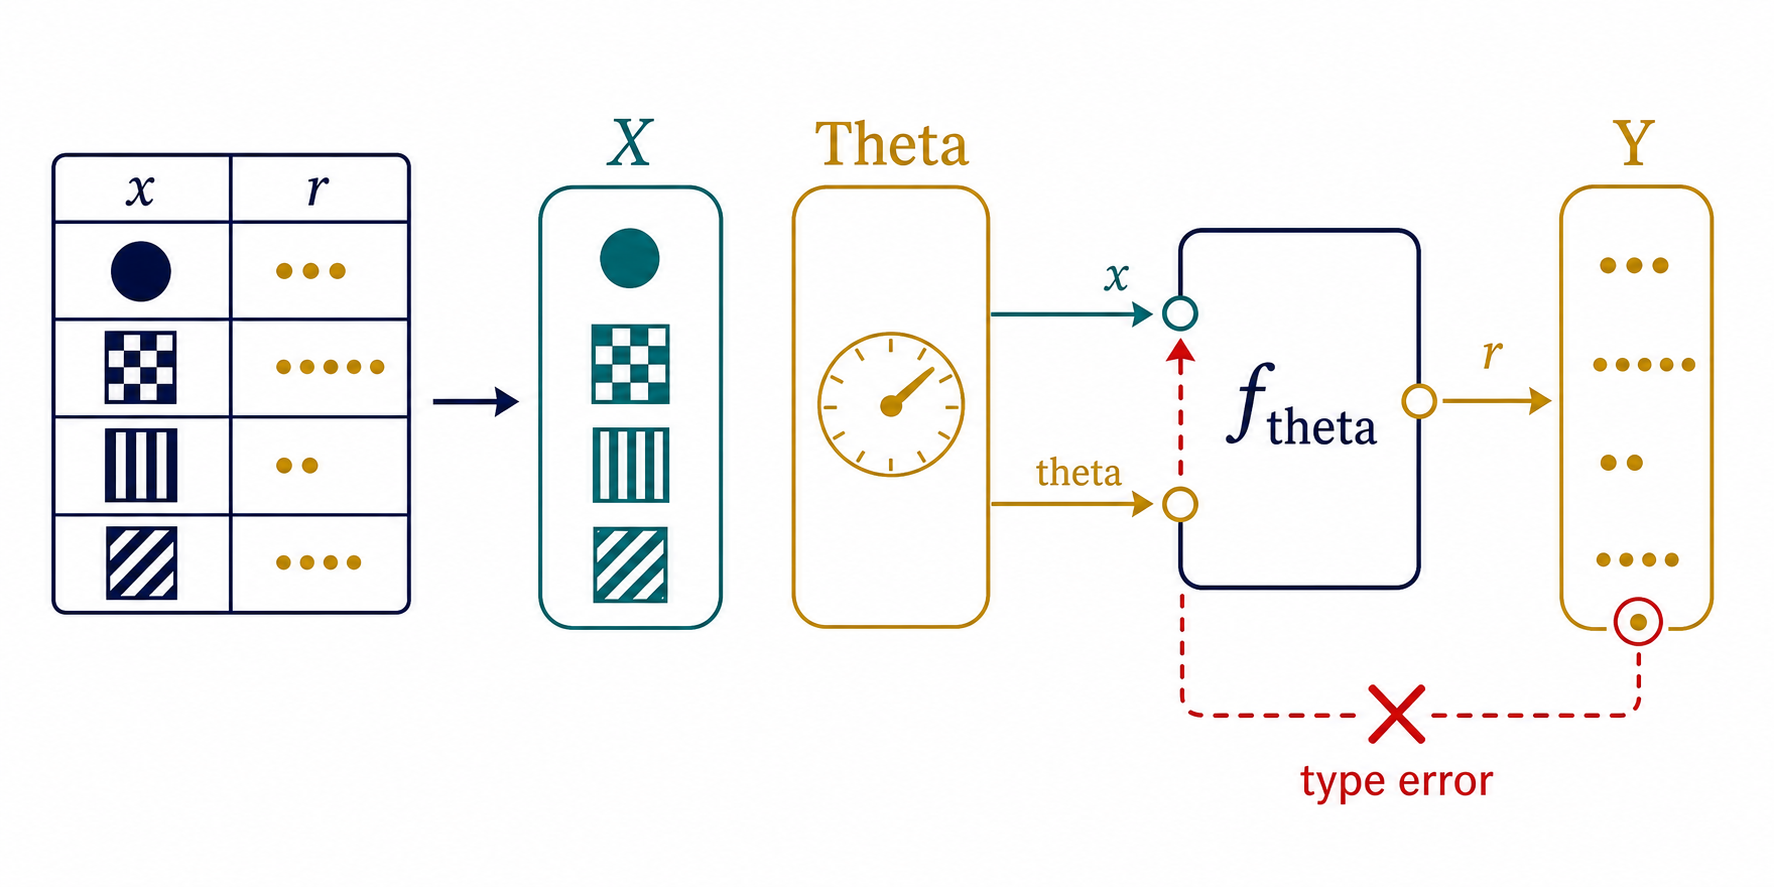
\includegraphics[width=0.94\linewidth]{imagegen-figures/ch01-typed-objects-statements-v4.png}
\caption{Typed notation separates data, valid inputs, parameters, and outputs. A stimulus \(x\in X\) and parameter \(\theta\in\Theta\) can enter the model \(f_\theta\), producing a response \(r\in Y\). The red dashed path shows a response object from \(Y\) being fed into the \(x\)-port: this is a type error, not merely a false statement.}
\label{fig:ch01-typed-objects-statements}
\end{figure}

\paragraph{Formal setup.}
Every symbol should come with a role. A common template is
\[
\theta\in\Theta,\qquad x\in X,\qquad f_\theta:X\to Y,\qquad r=f_\theta(x)\in Y.
\]
Here \(X\) is the domain, \(Y\) is the codomain, \(\Theta\) is a parameter space, \(x\) is an input variable, \(\theta\) is a fixed parameter, and \(r\) is an output. A central well-typed statement is
\[
\forall x\in X,\quad f_\theta(x)\in Y.
\]
The symbol \(\forall\) means "for all." The expression says that every allowed input produces an output of the promised kind. If we want to allow a stochastic model instead of a deterministic one, we change the object type:
\[
p_\theta(\,\cdot\mid x)\ \text{is a probability distribution on }Y\quad\text{for each }x\in X.
\]
The input \(x\) is still a stimulus object. The output is now a distribution over responses rather than a single response.

\paragraph{Core intuition.}
Notation is a system of labels and contracts. The labels tell us what each symbol names. The contracts tell us what operations are allowed. Figure~\ref{fig:ch01-typed-objects-statements} shows this visually: \(X\), \(\Theta\), \(Y\), and \(f_\theta\) are different objects with different ports. The model accepts a stimulus and a parameter. It returns a response. Feeding the response back into the stimulus port silently changes the problem unless a new map has been defined.

Common beginner mistakes are usually type mistakes in disguise. One is using the same letter for an object and its numerical representation. Another is changing a parameter inside a statement where it was assumed fixed. A third is treating a data point, a set of data points, and a distribution over data points as if they were interchangeable. The cure is not more symbols. The cure is a habit: write the domain, codomain, variables, parameters, and assumptions before manipulating the formula.

This section looks forward to Chapter 2, where functions become the first systematic typed relationships. It also looks forward to probability, where a random variable is not a random number floating in space but a function from outcomes to values.

\paragraph{Main derivation: type-checking a composed expression.}
Suppose
\[
f_\theta:X\to Y,\qquad \ell:Y\times Y\to\mathbb{R},\qquad x\in X,\qquad y\in Y.
\]
Then
\[
\ell(f_\theta(x),y)
\]
is well typed and is a real number. By contrast, \(\ell(x,y)\) is not well typed unless \(x\in Y\) or a different loss function has been defined on \(X\times Y\).

\emph{Derivation.} Start at the innermost expression. Since \(x\in X\) and \(f_\theta:X\to Y\), the value \(f_\theta(x)\) belongs to \(Y\). The ordered pair \((f_\theta(x),y)\) therefore belongs to \(Y\times Y\), the domain of \(\ell\). Because \(\ell:Y\times Y\to\mathbb{R}\), the expression \(\ell(f_\theta(x),y)\) belongs to \(\mathbb{R}\). Each step used a declared domain and codomain. That is the mechanism behind type-checking.

\paragraph{Worked examples.}
\emph{Small symbolic example.} Let \(X=\{a,b,c\}\), \(Y=\{0,1\}\), and define \(f:X\to Y\) by
\[
f(a)=0,\qquad f(b)=1,\qquad f(c)=1.
\]
The statement \(\forall x\in X,\ f(x)\in Y\) is true. The statement \(\forall x\in X,\ f(x)=1\) is false because \(f(a)=0\). The expression \(f(1)\) is ill typed because \(1\in Y\), not \(1\in X\), unless we separately declare that \(1\) is also an allowed input.

\emph{ML/neuroscience example.} In a supervised neural decoding problem, \(x\in X\) might be a vector of spike counts from \(100\) neurons, \(y\in Y\) might be a reach direction label, and \(f_\theta:X\to Y\) might be a trained decoder. The parameter \(\theta\) contains learned weights. The loss \(\ell(f_\theta(x),y)\) compares a predicted label with a true label. The objects map as follows: neural activity is the input object, the reach label is the output object, the decoder is the function, and the weights are parameters.

\paragraph{ML/DL/neuroscience connections.}
Deep learning frameworks enforce typed thinking through tensor shapes and module signatures. A linear layer may accept arrays of shape \(d\) and return arrays of shape \(k\); feeding a label vector into that layer is a type error. In neuroscience, a tuning curve, an encoding model, and a decoding model have different input-output types. A tuning curve maps stimuli to response summaries. A decoder maps neural responses to stimulus or behavior estimates. Confusing those directions leads to incorrect interpretation even when the formulas look similar.

\paragraph{Exercises.}
\begin{enumerate}[label=\textbf{1.1.\arabic*.}, leftmargin=*]
\item \textbf{Mechanical.} For \(X=\{\text{low},\text{high}\}\), \(Y=\{0,1,2\}\), and \(f:X\to Y\) with \(f(\text{low})=0\) and \(f(\text{high})=2\), identify the domain, codomain, input variable, and output values.
\item \textbf{Proof or derivation.} Let \(g:Y\to Z\) and \(f:X\to Y\). Prove by type-checking that \(g(f(x))\in Z\) for every \(x\in X\).
\item \textbf{Numerical/computational.} A model \(f_\theta:\mathbb{R}^3\to\mathbb{R}^2\) receives a vector of three neural features and returns two class scores. Decide whether each expression is well typed: \(f_\theta((1,0,4))\), \(f_\theta((1,0))\), and \(f_\theta(7)\).
\item \textbf{Interpretation.} In the notation \(p_\theta(\,\cdot\mid x)\), what object is fixed, what object varies, and what kind of object is returned?
\item \textbf{Debug the misconception.} A student says, "The equation \(f_\theta(r)=x\) is probably false." Explain why it may be worse than false: it may be meaningless unless the model has been typed to accept \(r\) as an input.
\end{enumerate}

\subsection{1.2 Sets, relations, and logical structure}

\paragraph{Motivating question.}
How do sets, relations, predicates, and quantifiers let us state exactly which objects are allowed, which objects are connected, and which claims are being made?

\paragraph{Beginner setup.}
A \emph{set} is a collection of objects. If \(a\) is an element of a set \(A\), we write \(a\in A\). If every element of \(C\) is also an element of \(A\), then \(C\subseteq A\). Sets give variables their allowed range.

A \emph{Cartesian product} \(A\times B\) is the set of ordered pairs \((a,b)\) with \(a\in A\) and \(b\in B\). A \emph{relation} from \(A\) to \(B\) is a subset \(R\subseteq A\times B\). If \((a,b)\in R\), then \(a\) is related to \(b\). Unlike a function, a relation may relate one object to many objects, many objects to one object, or no objects at all.

The smallest nontrivial example is
\[
A=\{a_1,a_2,a_3\},\qquad B=\{b_1,b_2\},
\]
with
\[
R=\{(a_1,b_1),(a_2,b_1),(a_2,b_2)\}\subseteq A\times B.
\]
The pair \((a_3,b_2)\) is a possible pair in \(A\times B\), but it is not in \(R\). A predicate is the statement form that selects the relation, such as \(P(a,b)\): "\(a\) evokes response category \(b\)."

What to keep in mind: sets specify where objects live; relations specify which pairs are selected; logic specifies how statements combine. This is the grammar underneath later phrases such as "for all inputs," "there exists a parameter," "stimuli are equivalent," and "this order preserves information."

\begin{figure}[htbp]
\centering
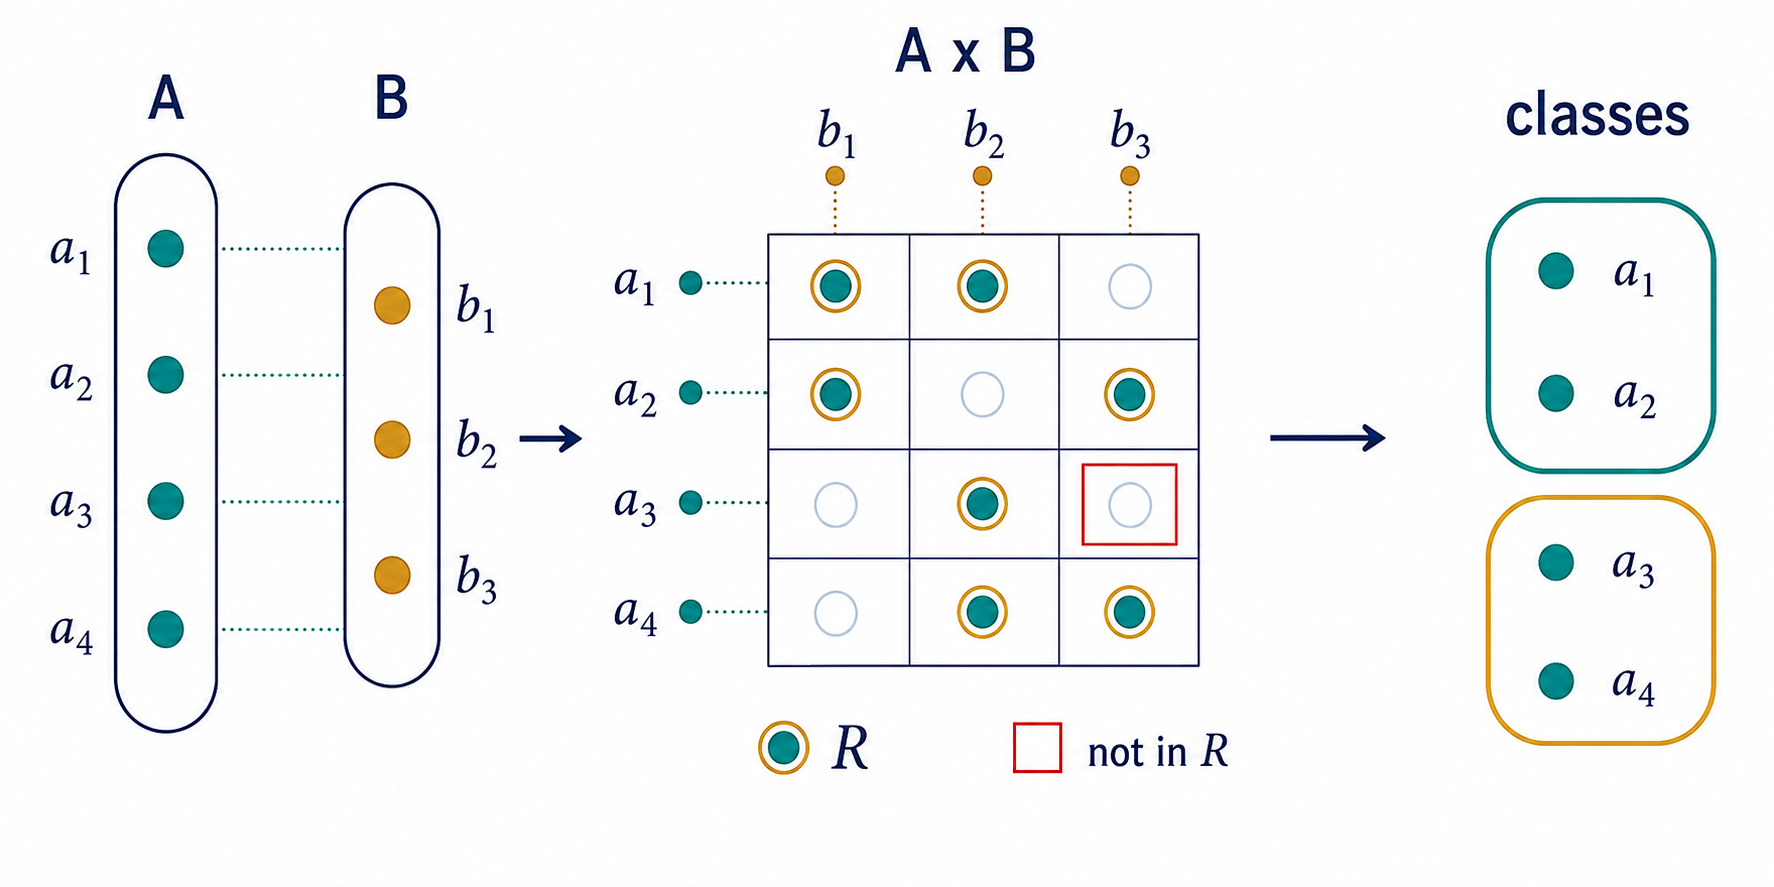
\includegraphics[width=0.94\linewidth]{imagegen-figures/ch01-sets-relations-classes-v2.png}
\caption{A relation is a selected subset of a Cartesian product. The middle grid represents possible pairs in \(A\times B\); highlighted cells belong to \(R\), while the red cell is a possible pair not chosen by the relation. The right panel shows how an equivalence relation on \(A\) groups elements into classes.}
\label{fig:ch01-sets-relations-classes}
\end{figure}

\paragraph{Formal setup.}
Let \(A\) and \(B\) be sets. A relation from \(A\) to \(B\) is
\[
R\subseteq A\times B.
\]
Equivalently, a predicate \(P(a,b)\) defines
\[
R=\{(a,b)\in A\times B:P(a,b)\text{ is true}\}.
\]
Logical connectives combine statements: \(P\wedge Q\) means both are true, \(P\vee Q\) means at least one is true, \(\neg P\) means \(P\) is false, and \(P\Rightarrow Q\) means whenever \(P\) holds, \(Q\) also holds. Quantifiers bind variables:
\[
\forall a\in A,\ P(a)
\qquad\text{and}\qquad
\exists a\in A\ \text{such that }P(a).
\]
An \emph{equivalence relation} on a set \(A\) is a relation \(\sim\) satisfying reflexivity, symmetry, and transitivity:
\[
a\sim a,\qquad a\sim b\Rightarrow b\sim a,\qquad (a\sim b\ \text{and}\ b\sim c)\Rightarrow a\sim c.
\]
A \emph{partial order} \(\preceq\) is a relation satisfying reflexivity, antisymmetry, and transitivity:
\[
a\preceq a,\qquad (a\preceq b\ \text{and}\ b\preceq a)\Rightarrow a=b,\qquad
(a\preceq b\ \text{and}\ b\preceq c)\Rightarrow a\preceq c.
\]

\paragraph{Core intuition.}
Figure~\ref{fig:ch01-sets-relations-classes} shows why a relation is more flexible than a function. The Cartesian product grid contains every possible pair. The relation selects some cells. A function is a special kind of relation that selects exactly one output cell in each input row. An equivalence relation is different: it relates objects in the same set and groups them into blocks. Those blocks are called equivalence classes.

The most common misconception is to read implication \(P\Rightarrow Q\) as if it said that \(P\) is true. It does not. It says that if \(P\) is true, then \(Q\) must be true. Another common mistake is swapping "for all" and "there exists." The statement "for every stimulus there exists a response" is much weaker than "there exists one response shared by every stimulus." In modeling, this difference can decide whether a claim is sensible.

This section builds the language that later chapters use constantly. A vector subspace is a subset closed under operations. A random variable uses preimages of sets. A metric is a relation-like rule for distances. A model class is a set of candidate functions. An equivalence relation is the formal version of treating several observations as the same for a chosen purpose.

\paragraph{Main theorem: equivalence relations partition a set.}
If \(\sim\) is an equivalence relation on \(A\), then the equivalence classes
\[
[a]=\{b\in A:b\sim a\}
\]
form a partition of \(A\): every element of \(A\) belongs to exactly one class, and two classes are either identical or disjoint. Conversely, any partition of \(A\) defines an equivalence relation by declaring two elements equivalent when they lie in the same block.

\emph{Proof sketch.} First, every \(a\in A\) belongs to its own class because \(a\sim a\) by reflexivity. So the classes cover \(A\). Now suppose two classes \([a]\) and \([c]\) overlap. Then some \(b\in A\) lies in both, so \(b\sim a\) and \(b\sim c\). By symmetry, \(a\sim b\). By transitivity, \(a\sim c\). If \(x\in[a]\), then \(x\sim a\), and since \(a\sim c\), transitivity gives \(x\sim c\). Thus \(x\in[c]\). The same argument in the other direction gives \([a]=[c]\). Therefore overlapping classes are identical, so distinct classes are disjoint.

For the converse, start with a partition of \(A\). Define \(a\sim b\) if \(a\) and \(b\) are in the same block. This is reflexive because every element is in its own block, symmetric because "same block" has no direction, and transitive because if \(a\) is in the same block as \(b\) and \(b\) is in the same block as \(c\), all three lie in one block.

\paragraph{Worked examples.}
\emph{Small numerical example.} On the integers \(\mathbb{Z}\), define \(m\sim n\) when \(m-n\) is divisible by \(3\). Then \(1\sim4\), \(2\sim5\), and \(0\sim6\). The equivalence classes are
\[
[0]=\{\ldots,-6,-3,0,3,6,\ldots\},
\]
\[
[1]=\{\ldots,-5,-2,1,4,7,\ldots\},
\]
\[
[2]=\{\ldots,-4,-1,2,5,8,\ldots\}.
\]
The relation compresses infinitely many integers into three remainder classes.

\emph{ML/neuroscience example.} Suppose \(A\) is a set of visual stimuli and define \(s\sim t\) if a trained classifier assigns the same label to \(s\) and \(t\). This is an equivalence relation if the classifier gives one label per stimulus. Its classes are decision regions. In neuroscience, define two trials equivalent if their spike-count vectors fall into the same response bin. Then an equivalence class is a response category: many detailed trials are treated as the same for the analysis.

\paragraph{ML/DL/neuroscience connections.}
A data set is usually a finite set of observations, labels, and metadata. A loss function selects relations between predictions and targets, such as "within tolerance" or "misclassified." A clustering algorithm produces an equivalence-like grouping of data points. A partial order appears when models are nested by complexity, when sigma-algebras are ordered by information, or when feature sets are ordered by inclusion. In each case, the mathematical object is not just a list of values. It is a set equipped with logical structure.

\paragraph{Exercises.}
\begin{enumerate}[label=\textbf{1.2.\arabic*.}, leftmargin=*]
\item \textbf{Mechanical.} Let \(A=\{1,2,3\}\), \(B=\{u,v\}\), and \(R=\{(1,u),(3,u),(3,v)\}\). List all elements of \(A\times B\), then identify which are in \(R\).
\item \textbf{Proof or derivation.} Prove that the relation \(m\sim n\) on \(\mathbb{Z}\), defined by " \(m-n\) is even," is an equivalence relation.
\item \textbf{Numerical/computational.} Given labels \(\text{cat},\text{dog},\text{cat},\text{bird},\text{dog}\) for five images, write the equivalence classes induced by "has the same label as."
\item \textbf{Interpretation.} If \(P(x)\) means "stimulus \(x\) evokes at least five spikes," explain the difference between \(\forall x\in X,\ P(x)\) and \(\exists x\in X\text{ such that }P(x)\).
\item \textbf{Debug the misconception.} A student says, "A relation from \(A\) to \(B\) must choose exactly one \(b\) for each \(a\)." Explain why that describes a function, not a general relation.
\end{enumerate}

\subsection{1.3 Proof methods and mathematical maturity}

\paragraph{Motivating question.}
Given a claim such as "if \(P\), then \(Q\)," how do we choose a proof method that actually addresses the logical shape of the claim?

\paragraph{Beginner setup.}
A \emph{proof} is a chain of justified statements that shows a conclusion follows from assumptions and definitions. It is not a performance of cleverness. It is an audit trail. A reader should be able to see where each step came from.

The smallest nontrivial proof target is an implication:
\[
P\Rightarrow Q.
\]
A direct proof assumes \(P\) and derives \(Q\). A contrapositive proof proves \(\neg Q\Rightarrow \neg P\), which is logically equivalent. A contradiction proof assumes \(P\) and \(\neg Q\) together and derives an impossibility. A counterexample refutes a universal claim by giving one allowed object where it fails. A construction proof proves existence by building an object. Induction proves a statement for natural numbers by proving a base case and a step from \(n\) to \(n+1\).

What to keep in mind: proof methods are not rituals. They are ways of matching your work to the failure case of the claim. For \(P\Rightarrow Q\), the only way the implication can fail is if \(P\) is true and \(Q\) is false.

\begin{figure}[htbp]
\centering
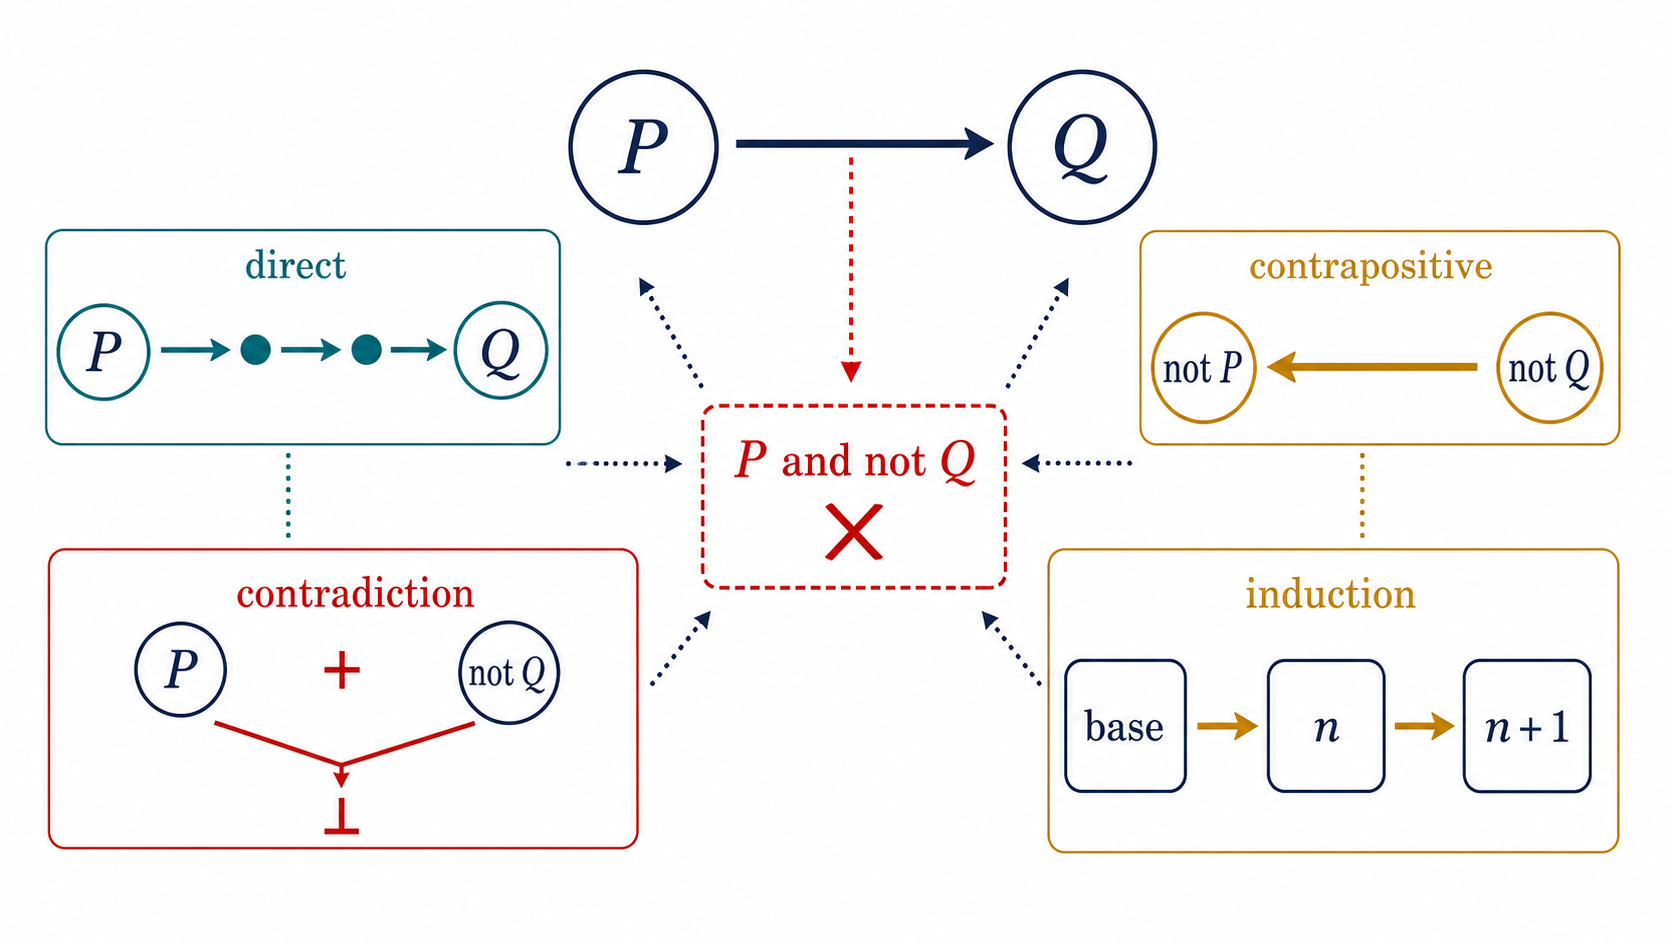
\includegraphics[width=0.92\linewidth]{imagegen-figures/ch01-proof-methods-v2.png}
\caption{Common proof methods reorganize the same implication. Direct proof builds a path from \(P\) to \(Q\); contrapositive starts from \(\neg Q\); contradiction occupies and destroys the failure case \(P\wedge\neg Q\); induction propagates a base case forward.}
\label{fig:ch01-proof-methods}
\end{figure}

\paragraph{Formal setup.}
Let \(P\) and \(Q\) be statements about objects in a specified domain \(D\). The implication
\[
\forall x\in D,\quad P(x)\Rightarrow Q(x)
\]
means that no object \(x\in D\) has \(P(x)\) true and \(Q(x)\) false:
\[
\{x\in D:P(x)\ \text{and}\ \neg Q(x)\}=\emptyset.
\]
This empty-failure-set equation is the central formal idea. Different proof methods show emptiness in different ways. Direct proof transforms \(P(x)\) into \(Q(x)\). Contrapositive proof transforms \(\neg Q(x)\) into \(\neg P(x)\). Contradiction assumes membership in the failure set and derives an impossibility. Counterexample finds a member of the failure set, thereby showing the universal implication is false.

\paragraph{Core intuition.}
Figure~\ref{fig:ch01-proof-methods} places the failure case in the center. If you can rule out \(P\wedge\neg Q\), the implication stands. Direct proof is often best when \(Q\) is easy to calculate from \(P\). Contrapositive proof is often best when the negation of \(Q\) has a useful algebraic form. Contradiction is useful when the assumptions force two incompatible facts. Induction is useful when the domain has a recursive structure: prove the first tile, then prove each tile knocks down the next.

Common misconceptions are predictable. First, examples do not prove universal claims, though they can guide a proof. Second, a proof by contradiction must derive a genuine impossibility, not merely an inconvenient result. Third, a counterexample must satisfy all assumptions. Fourth, definitions are not optional: many proof steps are simply the correct unpacking of a definition.

This section prepares students for later chapters where proofs justify computational shortcuts. Projection formulas, rank-nullity, Taylor approximation, Bayes' theorem, concentration bounds, and information identities are all easier to learn when the proof method matches the claim.

\paragraph{Main theorem: three proof forms for implication agree.}
For statements \(P\) and \(Q\), the following are equivalent:
\[
P\Rightarrow Q,\qquad \neg Q\Rightarrow \neg P,\qquad \neg(P\wedge\neg Q).
\]

\emph{Proof sketch.} The implication \(P\Rightarrow Q\) fails only in one situation: \(P\) is true and \(Q\) is false. Therefore saying \(P\Rightarrow Q\) is the same as saying not both \(P\) and \(\neg Q\). That gives \(P\Rightarrow Q\) equivalent to \(\neg(P\wedge\neg Q)\).

Now compare \(P\Rightarrow Q\) with its contrapositive. If \(P\Rightarrow Q\) is true and \(\neg Q\) holds, then \(P\) cannot hold, because \(P\) would force \(Q\). Thus \(\neg P\) holds. So \(\neg Q\Rightarrow\neg P\). Conversely, if \(\neg Q\Rightarrow\neg P\) is true and \(P\) holds, then \(\neg Q\) cannot hold, because it would force \(\neg P\). Hence \(Q\) holds. The mechanisms are different, but the logical content is the same.

\paragraph{Worked examples.}
\emph{Small symbolic example.} Claim: for every integer \(n\), if \(n\) is even, then \(n^2\) is even. A direct proof starts by unpacking the definition of even: \(n=2k\) for some integer \(k\). Then
\[
n^2=(2k)^2=4k^2=2(2k^2),
\]
so \(n^2\) is even. A contrapositive proof would show that if \(n^2\) is odd, then \(n\) is odd. Both approaches target the same implication.

Counterexample example: the statement "for every integer \(n\), if \(n^2\) is even, then \(n\) is divisible by \(4\)" is false. Let \(n=2\). Then \(n^2=4\) is even, but \(n\) is not divisible by \(4\). The counterexample satisfies the assumption and violates the conclusion.

\emph{ML/neuroscience example.} Consider a deterministic threshold classifier
\[
f(x)=
\begin{cases}
1,& \operatorname{score}(x)\ge t,\\
0,& \operatorname{score}(x)<t.
\end{cases}
\]
The claim "if \(f(x)=1\), then \(\operatorname{score}(x)\ge t\)" is proved by reading the definition of \(f\). The objects map as follows: \(x\) is an input trial or stimulus, \(\operatorname{score}(x)\) is a real-valued feature computed by the model, \(t\) is a parameter, and \(f(x)\) is the predicted class. A proof about the classifier is not a vague argument about performance; it is a statement about how the prediction rule was defined.

\paragraph{ML/DL/neuroscience connections.}
In machine learning, many claims are conditional: if the loss is convex, then a local minimizer is global; if a matrix has full column rank, then least-squares coefficients are unique; if two variables are conditionally independent, then a factorization is valid. In neuroscience, a model may imply a qualitative prediction: if two stimuli lie in the same equivalence class of a representation, then the decoder cannot distinguish them using that representation alone. Proof tells us what follows from the model assumptions before we ask whether the assumptions match biology.

\paragraph{Exercises.}
\begin{enumerate}[label=\textbf{1.3.\arabic*.}, leftmargin=*]
\item \textbf{Mechanical.} For the claim "if \(n\) is divisible by \(6\), then \(n\) is divisible by \(3\)," identify \(P\), \(Q\), the contrapositive, and the failure case.
\item \textbf{Proof or derivation.} Prove directly that if \(a\) and \(b\) are even integers, then \(a+b\) is even.
\item \textbf{Numerical/computational.} Search the integers \(n=-5,-4,\ldots,5\) for a counterexample to the statement "if \(n^2>4\), then \(n>2\)." Report the first counterexample and explain which assumption and conclusion it satisfies or violates.
\item \textbf{Interpretation.} A theorem says, "If the design matrix has full column rank, then the least-squares solution is unique." What must you check before using the theorem on a data set?
\item \textbf{Debug the misconception.} A student gives three examples where a universal claim is true and says the claim is proved. Explain what examples can and cannot establish.
\end{enumerate}

\subsection{1.4 Mathematical modeling as compression}

\paragraph{Motivating question.}
When a mathematical model replaces a messy experiment with variables, equations, and parameters, what information is being kept, what is being discarded, and why can the compression still be useful?

\paragraph{Beginner setup.}
A \emph{mathematical model} is a simplified structure used to predict, explain, or organize phenomena. It does not copy reality. It compresses reality by choosing state variables, relations, parameters, and loss functions. A good model keeps information relevant to its purpose and discards details that are irrelevant, unavailable, or too expensive to use.

The smallest nontrivial example is a stimulus-response table. Suppose four stimuli have measured average spike counts:
\[
\begin{array}{c|cccc}
\text{stimulus} & x_1 & x_2 & x_3 & x_4\\
\hline
\text{mean count} & 2 & 3 & 9 & 10
\end{array}
\]
A lookup-table model stores all four numbers. A compressed model might store only whether the stimulus has low or high contrast:
\[
\pi(x_1)=\pi(x_2)=\text{low},\qquad \pi(x_3)=\pi(x_4)=\text{high},
\]
with predictions \(m(\text{low})=2.5\) and \(m(\text{high})=9.5\). This loses stimulus-level detail but preserves the main response difference.

What to keep in mind: abstraction is not vagueness. A compressed model should say exactly what map compresses the observations, what model acts on the compressed state, what prediction is produced, and how error is measured.

\begin{figure}[htbp]
\centering
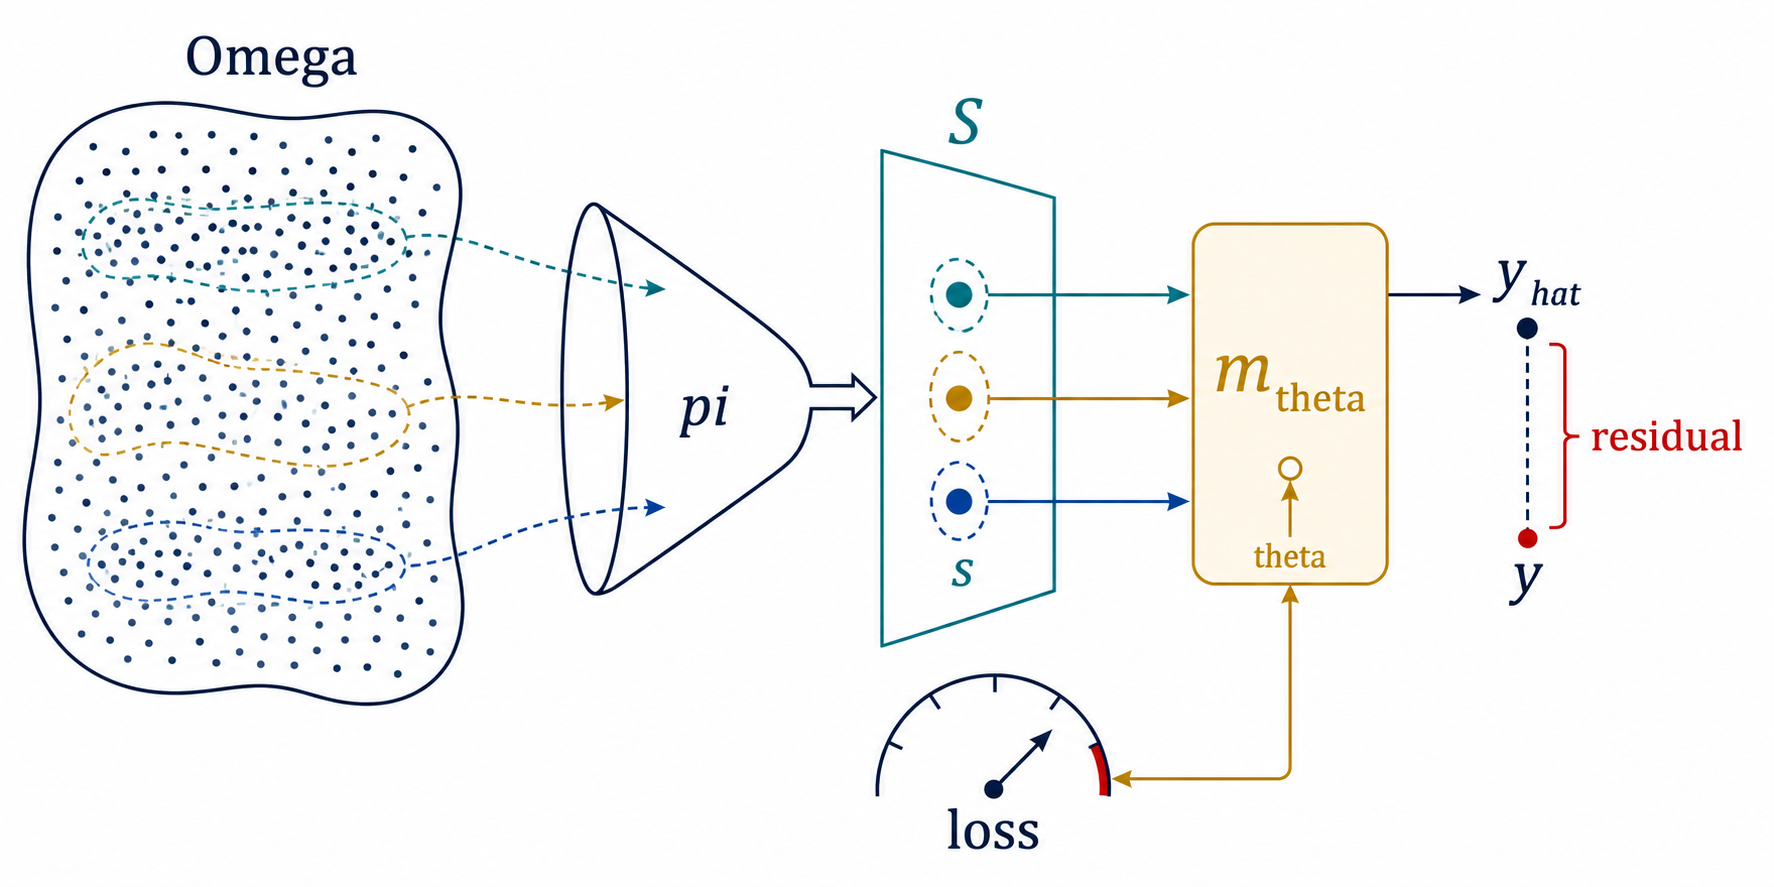
\includegraphics[width=0.94\linewidth]{imagegen-figures/ch01-modeling-compression-v2.png}
\caption{Modeling as compression. Fibers in \(\Omega\) show groups of observations treated as equivalent by \(\pi\). The compact state \(s\in S\) feeds \(m_\theta\), while the residual between \(\hat y\) and \(y\) sends information back through the loss.}
\label{fig:ch01-modeling-compression}
\end{figure}

\paragraph{Formal setup.}
Let \(\Omega\) be a raw observation space. An observation \(\omega\in\Omega\) may contain many details: stimulus identity, time, neural activity, behavior, noise, and metadata. A representation map
\[
\pi:\Omega\to S
\]
compresses \(\omega\) into a state \(s=\pi(\omega)\) in a smaller or more structured state space \(S\). A model with parameter \(\theta\in\Theta\) maps state to prediction:
\[
m_\theta:S\to Y,\qquad \hat y=m_\theta(\pi(\omega)).
\]
Given training pairs \((\omega_i,y_i)\) and a loss \(\ell:Y\times Y\to\mathbb{R}_{\ge 0}\), fitting often means solving
\[
\min_{\theta\in\Theta}\ \sum_{i=1}^n \ell\!\left(m_\theta(\pi(\omega_i)),y_i\right).
\]
The dimensions and types matter: \(\omega_i\in\Omega\), \(\pi(\omega_i)\in S\), \(m_\theta(\pi(\omega_i))\in Y\), \(y_i\in Y\), and the loss is a nonnegative number.

\paragraph{Core intuition.}
Figure~\ref{fig:ch01-modeling-compression} shows compression as fibers. A fiber of \(\pi\) is a set of raw observations that map to the same state:
\[
\pi^{-1}(\{s\})=\{\omega\in\Omega:\pi(\omega)=s\}.
\]
Inside a fiber, the model treats observations as equivalent for its current purpose. That may be wise or foolish. If the discarded details do not help predict \(y\), the compression is efficient. If the discarded details contain important information, the model will make systematic errors.

Common misconceptions: first, a more detailed model is not automatically better. A lookup table can memorize but fail to generalize. Second, a simpler model is not automatically more scientific. It may discard the very variable that matters. Third, fitting a model is not the same as validating it. A model can fit the training data while compressing the wrong structure.

This section connects backward to equivalence classes: a representation map groups raw observations into classes. It connects forward to functions, coordinates, projections, sufficient statistics, latent variables, probabilistic models, and information theory.

\paragraph{Main derivation: when compression is predictively sufficient.}
Suppose the target \(y\) is generated from raw observations \(\omega\), and a representation \(\pi:\Omega\to S\) satisfies
\[
p(y\mid \omega)=p(y\mid \pi(\omega))
\]
for all relevant \(\omega\) and \(y\). Then \(\pi(\omega)\) preserves all information in \(\omega\) needed for predicting \(y\).

\emph{Derivation.} The left side is the predictive distribution available if the model knows the full raw observation \(\omega\). The right side is the predictive distribution available if the model knows only the compressed state \(s=\pi(\omega)\). If the two are equal for every case, then replacing \(\omega\) by \(\pi(\omega)\) does not change any prediction about \(y\). In other words, all observations in the same fiber of \(\pi\) have the same target-relevant predictive distribution. The compression may lose details about lighting, trial number, or exact waveform shape, but by assumption those details do not change the conditional distribution of the target.

This is a mechanism, not a magic guarantee. In practice we rarely know the equality exactly. We choose \(\pi\), fit \(m_\theta\), and test whether the residuals reveal discarded structure.

\paragraph{Worked examples.}
\emph{Small numerical example.} Return to the four-stimulus table. The lookup table predictions are \(2,3,9,10\), so it stores four response values. The contrast-compressed model stores two states and two predictions: low maps to \(2.5\), high maps to \(9.5\). Its squared errors are
\[
(2.5-2)^2+(2.5-3)^2+(9.5-9)^2+(9.5-10)^2=1.
\]
The model has compressed four stimulus identities into two state values with small error. If the table had been \(2,10,3,9\), the same compression would have large error because contrast would no longer explain the response pattern.

\emph{ML/neuroscience example.} In image classification, \(\omega\) may be a full image, \(\pi(\omega)\) may be an embedding produced by a neural network trunk, \(m_\theta\) may be a linear classifier on the embedding, and \(y\) may be the class label. The embedding compresses pixels into features. In neuroscience, \(\omega\) may be a raw spike train from many neurons over a trial, \(\pi(\omega)\) may be a vector of binned firing rates or a low-dimensional latent state, \(m_\theta\) may predict movement direction, and \(y\) is the observed behavior. The mathematical objects are raw observation, representation, state space, model, prediction, target, residual, and loss.

\paragraph{ML/DL/neuroscience connections.}
Representation learning is learned compression. Autoencoders compress inputs into latent codes and reconstruct them. Decoders compress neural population activity into behavioral predictions. Encoding models compress stimuli into features that explain responses. Bayesian models compress data into posterior distributions over parameters. Later, PCA will compress data by preserving variance, sufficient statistics will compress data without losing information about a parameter, and information theory will quantify how much uncertainty a representation removes.

\paragraph{Exercises.}
\begin{enumerate}[label=\textbf{1.4.\arabic*.}, leftmargin=*]
\item \textbf{Mechanical.} In the pipeline \(\omega\mapsto \pi(\omega)=s\mapsto m_\theta(s)=\hat y\), identify the raw observation space, state space, model, parameter, prediction, and target.
\item \textbf{Proof or derivation.} Suppose \(\pi(\omega_1)=\pi(\omega_2)\) and \(p(y\mid\omega)=p(y\mid\pi(\omega))\). Show that \(p(y\mid\omega_1)=p(y\mid\omega_2)\).
\item \textbf{Numerical/computational.} For response values \(1,2,8,9\), compress the first two observations into state \(a\) and the last two into state \(b\). Use the mean response within each state as the prediction and compute the total squared error.
\item \textbf{Interpretation.} In a neural decoding study, what might be gained and what might be lost by replacing raw spike trains with binned spike counts?
\item \textbf{Debug the misconception.} A student says, "A model with more variables is always less abstract and therefore more accurate." Explain why additional variables can improve, harm, or leave unchanged the quality of prediction.
\end{enumerate}

Chapter 1 has treated mathematical language as a disciplined way to compress thought: objects have types, statements have assumptions, proofs rule out failure cases, and models compress observations for a purpose. Chapter 2 turns the first of these habits into a central object of study. Once we know the allowed inputs and outputs, a function becomes a typed relationship between them, and coordinate systems become ways of representing those objects for computation.

\clearpage
